
%%%%%%%%%%%%%%%%%%%%%%%%%%%%%%%%%%%%%%
\documentclass{article}
\usepackage{Sweave}
\usepackage{graphicx}
\usepackage{tabularx}
\usepackage{natbib}
\usepackage{pdflscape}
\usepackage{array}
\usepackage{textcomp, gensymb}
\usepackage{amsmath}
\usepackage{longtable}
\usepackage{xr}
\usepackage[small]{caption}
\usepackage{xr-hyper} %refer to Fig.s in another document
%\usepackage{hyperref}

\setkeys{Gin}{width=0.8\textwidth}
\setlength{\captionmargin}{30pt}
\setlength{\abovecaptionskip}{10pt}
\setlength{\belowcaptionskip}{10pt}
 \topmargin -1.5cm        
 \oddsidemargin -0.04cm   
 \evensidemargin -0.04cm
 \textwidth 16.59cm
 \textheight 21.94cm 
 \parskip 7.2pt          
 \parindent 0pt
\usepackage{setspace}
%\externaldocument{PhenoPhylo_ms_submit}
\externaldocument{PhenoPhylo_ms_submit_wbib}
\externaldocument{PhenoPhylo_SuppMat_submit}
%%%%%%%%%%%%%%%%%%%%%%%%%%%%%%%%%%%%%%

\begin{document}

%\bibliographystyle{naturemag}
\title{Extended Data Phylogenetic estimates of species-level phenology improve ecological forecasting} 

\author{Ignacio Morales-Castilla,$^{1}$ T. J. Davies,$^{2,3}$ Geoffrey Legault,$^{3}$ D. M. Buonaiuto,$^{4,5,6}$ \\ Catherine J. Chamberlain,$^{4,5,7}$ Ailene K. Ettinger,$^{5,8}$ Mira Garner,$^{3}$ Faith A. M. Jones,$^{3,10}$ \\ Deirdre Loughnan,$^{3}$ William D. Pearse,$^{11}$ Darwin S. Sodhi$^{3}$ \\\& E. M. Wolkovich$^{3,4,5}$ }


 
\maketitle  
%%%%%%%%%%%%%%%%%%%%%%%%%%%%%%%%%%%%%%%%%%%%%%%%%%%
\renewcommand{\thefigure}{Extended Data \arabic{figure}}





\begin{figure}
\centering
  \noindent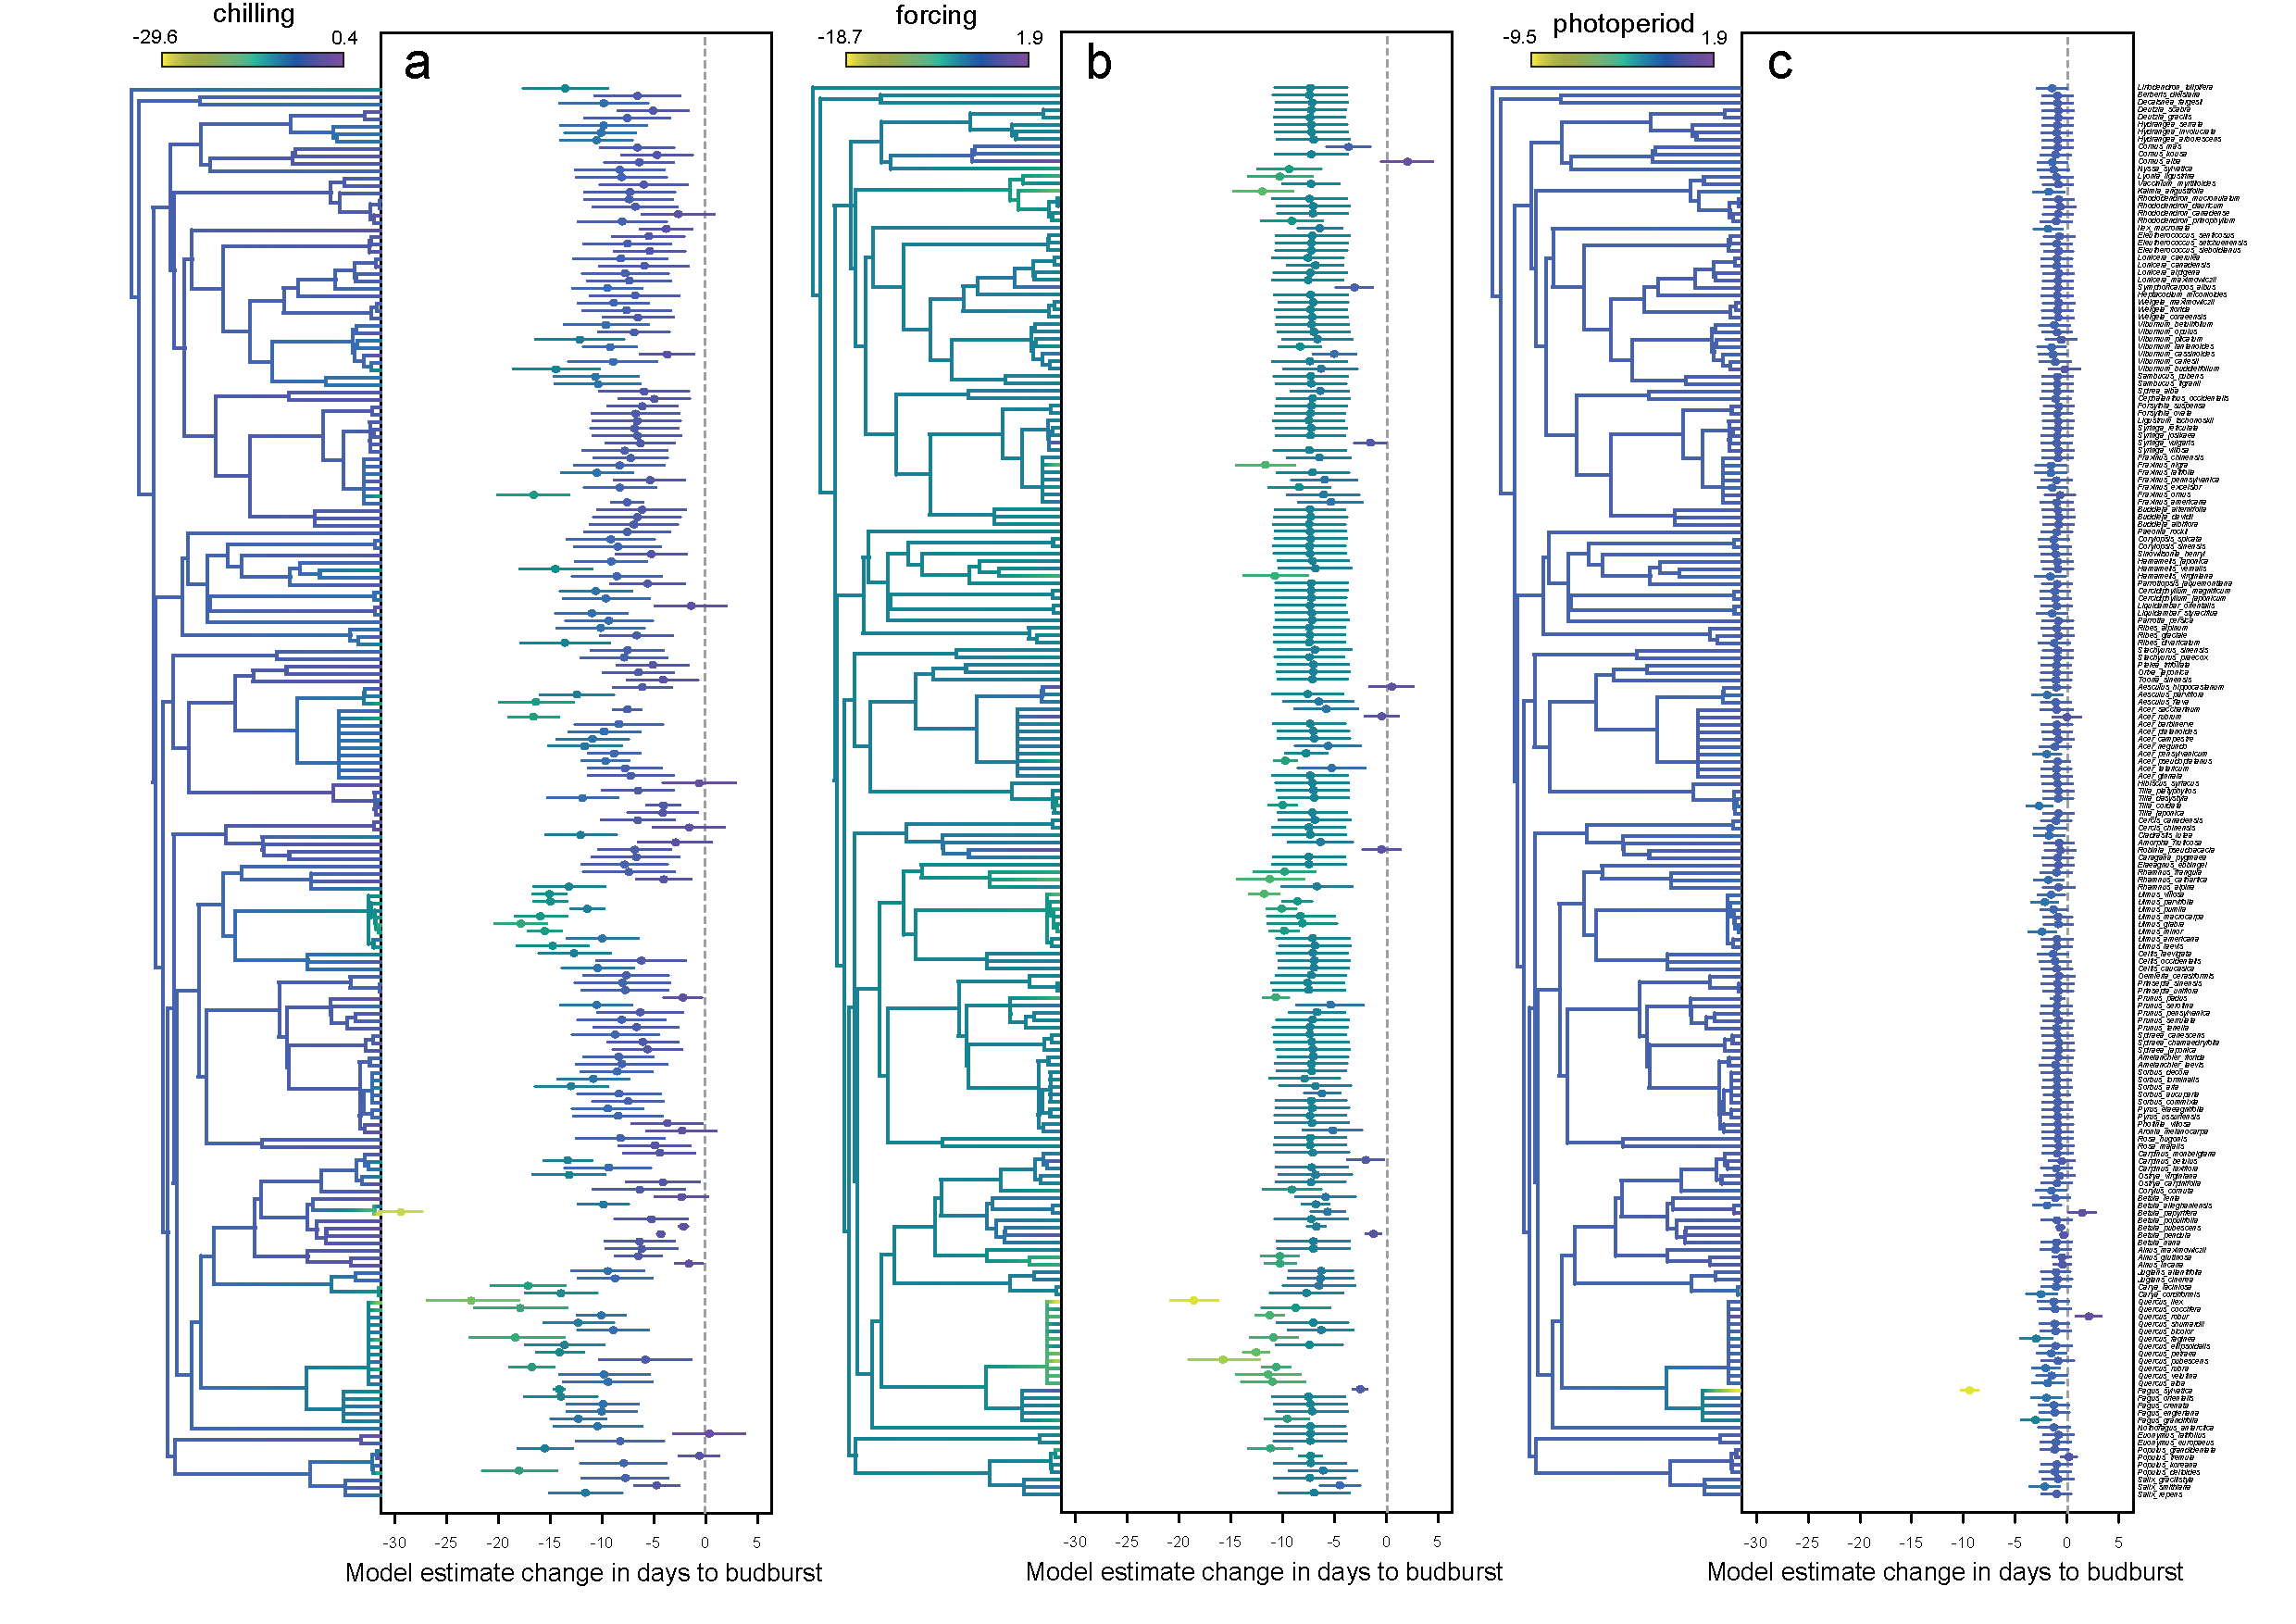
\includegraphics[width=0.9\textwidth]{../../analyses/phylogeny/figures/FigSXX_ phylo_muplots191_lamb0.pdf}
  \caption{\textbf{Phenological sensitivity to three environmental cues across 191 woody species estimated by a non-phylogenetic Hierarchical Mixed Model.} Non-phylogenetic phenological sensitivity to three environmental cues, chilling (a), forcing (b) and photoperiod (c) measured in change in days to budburst per standardized unit (z-transformation) of the cues across 191 tree species. Sensitivity estimates are computed by commonly used hierarchical model where phylogenetic distances are not accounted for ($\lambda$ = 0). The database used to fit the model comprised 44 studies, 191 species and 2940 observations. The same phylogenetic tree is shown in each panel, colored according to an estimation of ancestral character states, being the states at the tips the species' sensitivities to a cue. Species sensitivities are shown as mean values $+/-$ 50\% uncertainty Intervals in the diagrams. Note that the color scale varies in each panel. Total tree depth is 81. My.}
  \label{fig:suppmuplot_all} 
\end{figure}

\clearpage


\begin{figure}
\centering
\noindent \includegraphics[width=0.9\textwidth]{../../analyses/phylogeny/figures/Figsupp_forecasting_maps_pngnice_virid.pdf}
  \caption{\textbf{Comparison of phenological forecasts by phylogenetic and non-phylogenetic models} Maps comparing projections of phylogenetic (PMM) against non-phylogenetic (HMM) models into the European distributions of two overlapping species, one well represented in the dataset \emph{Betula pendula} (a) and one underrepresented \emph{Acer campestre} (b). The color scale shown in maps and histograms reflects budbreak differences between models where days are relative to start of forcing conditions, not calendar days.}
  \label{fig:pmmvshmm}
\end{figure}
\clearpage


\begin{figure}
  \centering
\noindent 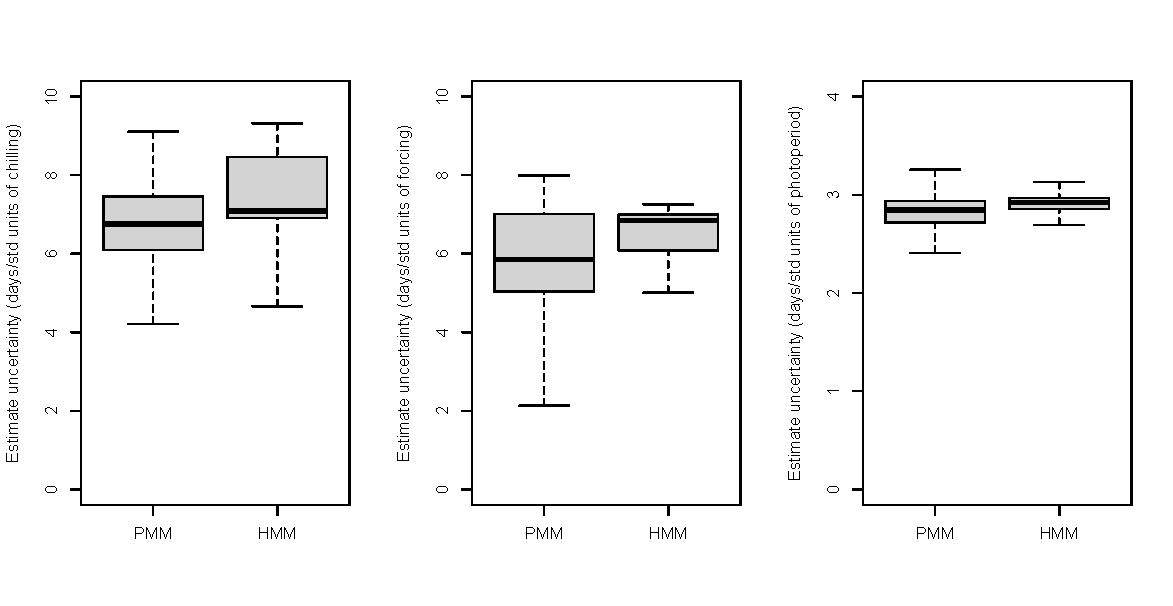
\includegraphics[width=0.9\textwidth]{../../analyses/phylogeny/figures/FigSXX_cue_uncert_lambest0.pdf}
  \caption{\textbf{Comparison of uncertainty around cue sensitivities estimated by the phylogenetic and non-phylogenetic models} Species uncertainties in model estimation of sensitivity to chilling (a), forcing (b) and photoperiod (c) of individual species between the phylogenetic model with estimated $\lambda$ (PMM), and the non-phylogenetic model with $\lambda$ = 0 (HMM). The non-phylogenetic model increases uncertainty. Box plots are calculated for ($n = 191$) uncertainty measurements corresponding to each species in our dataset. Box upper and lower limits represent the first and third quartiles (25th and 75th percentiles, respectively), the median is represented as the horizontal line internal to the box and whiskers reach 1.5 times the interquartile range.}
  \label{fig:suppuncertainties}
\end{figure}
\clearpage


\begin{figure}
  \centering
\noindent 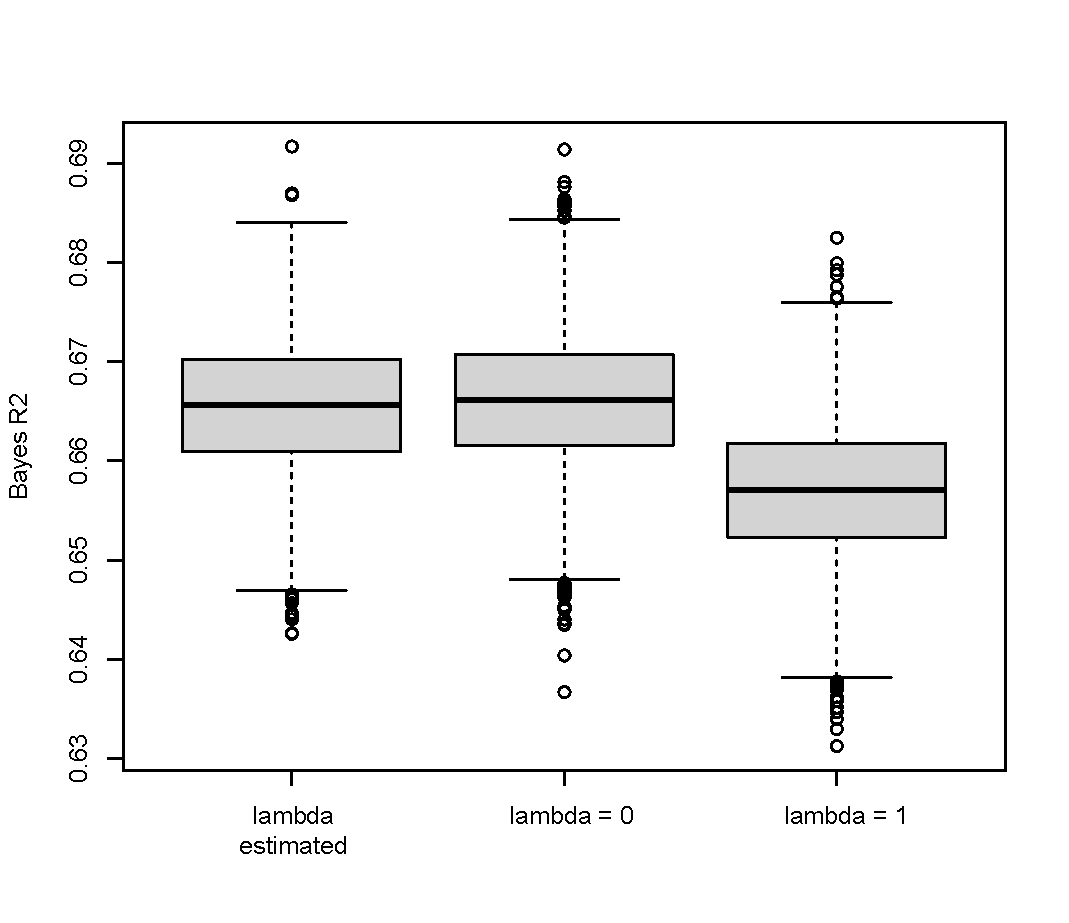
\includegraphics[width=0.9\textwidth]{../../analyses/phylogeny/figures/Boxplot_bayesR2.pdf}
  \caption{\textbf{Comparison of overall model accuracy between the phylogenetic model and the non-phylogenetic model.} Accuracy is measured by Bayes \emph{R\textsuperscript{2}}. There are no differences in accuracy even if individual species estimates markedly differ between models. Bayes \emph{R\textsuperscript{2}} was computed across the posterior distributions of predicted values for each model (effective sample size is, $n = 636$ for PMM and $n = 649$ for HMM). Box upper and lower limits represent the first and third quartiles (25th and 75th percentiles, respectively), the median is represented as the horizontal line internal to the box and whiskers reach 1.5 times the interquartile range.}
  \label{fig:accuracycomp}
\end{figure}
\clearpage

\begin{figure}
  \centering
\noindent 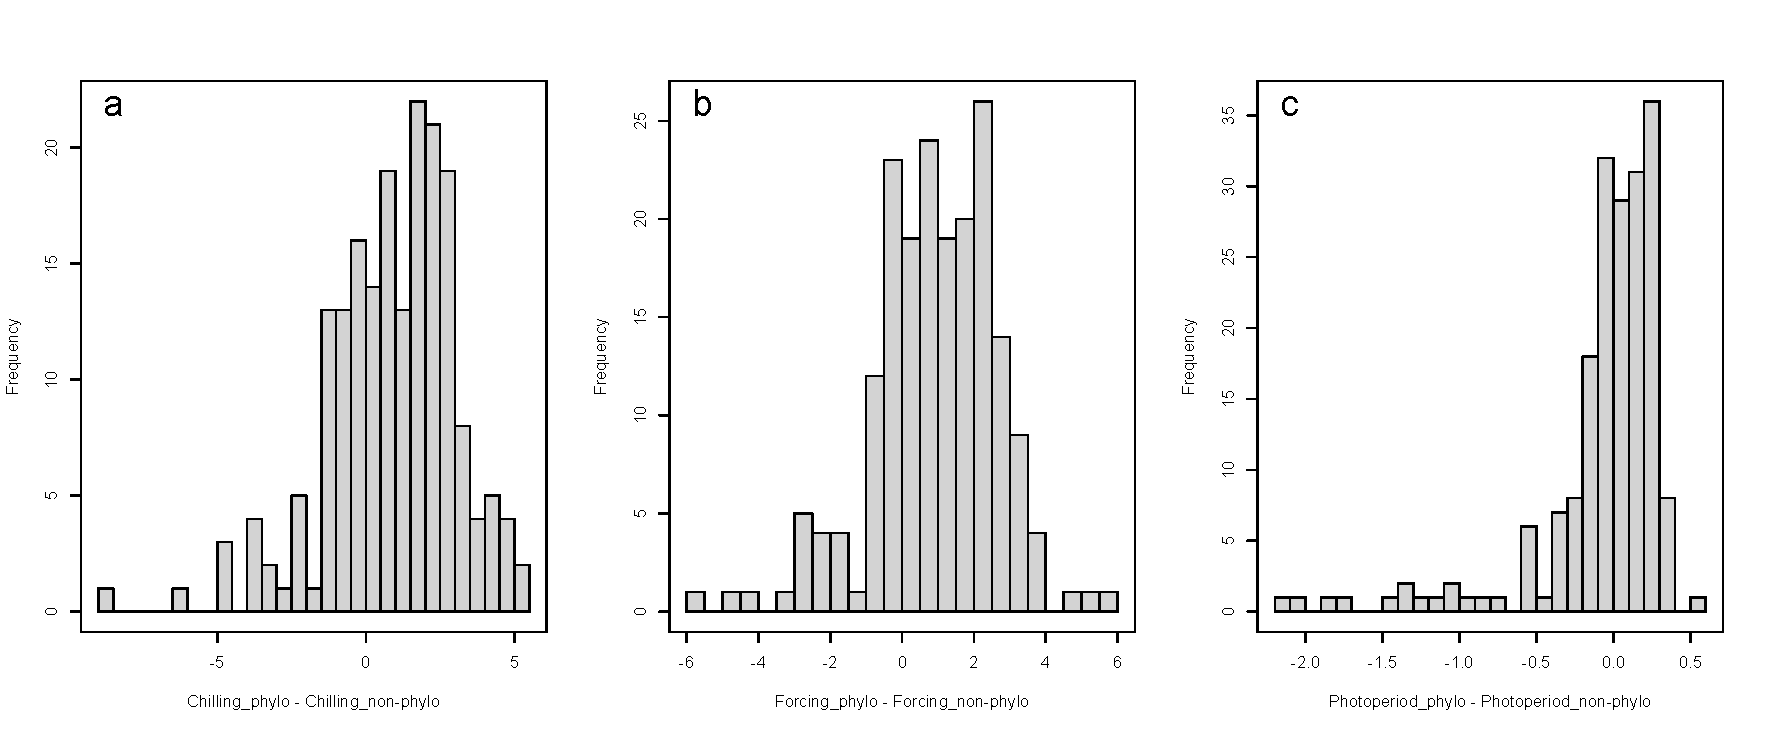
\includegraphics[width=0.9\textwidth]{../../analyses/phylogeny/figures/FigSXX_bias_sens_phylo_nonphylo.pdf}
  \caption{\textbf{Comparison of observed vs. predicted values of days to budburst for held out species in cross-validation analyses.} Predicted values for days to budburst are modelled by the more traditional hierarchical mixed model (HMM; panel a) and the phylogenetic mixed model we present (PMM; panel b). Observed and predicted values according to the leave-one-clade-out scheme (see Extended Methods section in Supplementary Information) were for the 2435 observations belonging to the 112 species in the 25 genera with more records.}
  \label{fig:biasestimation}
\end{figure}
\clearpage


\begin{figure}
  \centering
\noindent 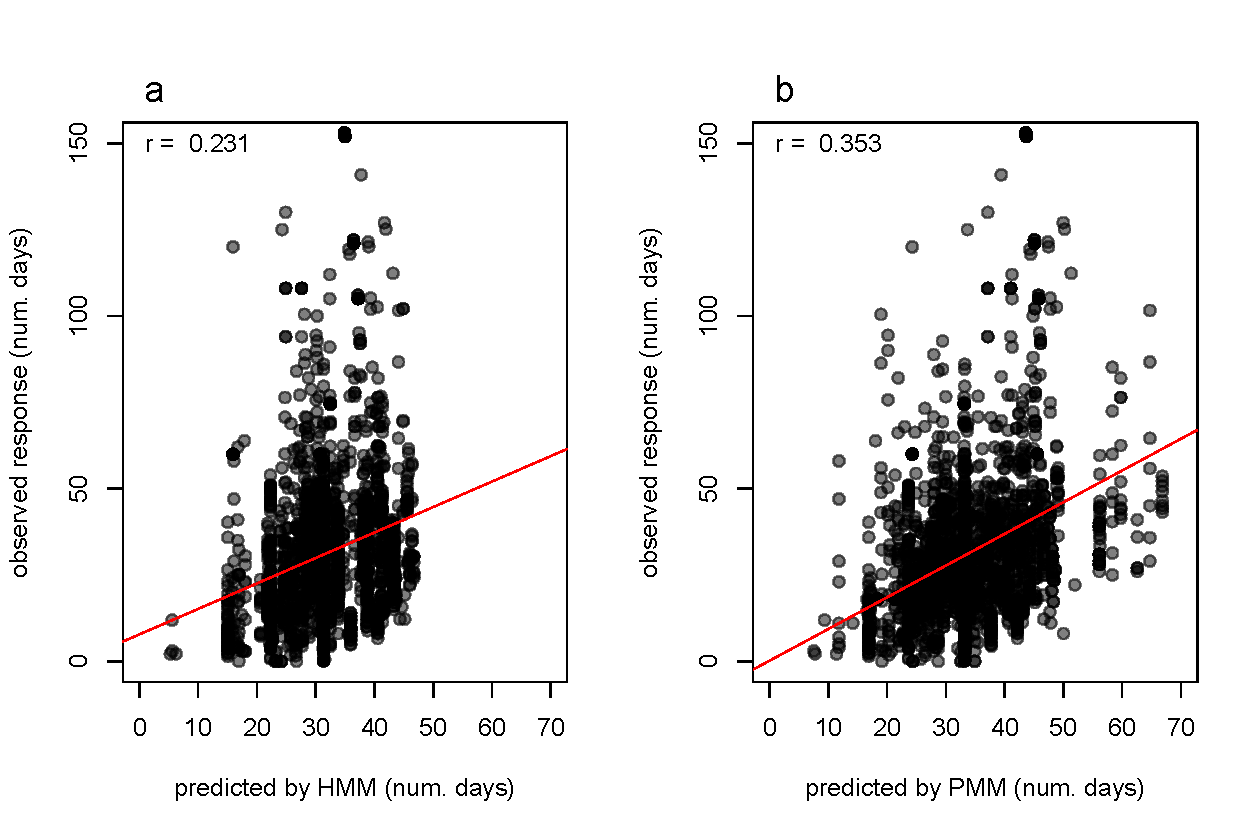
\includegraphics[width=0.9\textwidth]{../../analyses/phylogeny/figures/FigSXXX_LOCO_observed_vs_predicted}
  \caption{\textbf{Comparison of correlations between cue sensitivities based on a leave-one-clade-out cross validation.} Correlations are computed between estimated slopes for species in subset models after leaving out a genus, and the full model including forcing as the predictor, for both the phylogenetic mixed model (PMM) and the hierarchical mixed model (HMM). Box plots are computed across ($n = 25$) iterations where one genus with at least 2 species was left out. Box upper and lower limits represent the first and third quartiles (25th and 75th percentiles, respectively), the median is represented as the horizontal line internal to the box and whiskers reach 1.5 times the interquartile range.}
  \label{fig:LOCO_obsvspred} 
\end{figure}
\clearpage

\begin{figure}
  \centering
\noindent 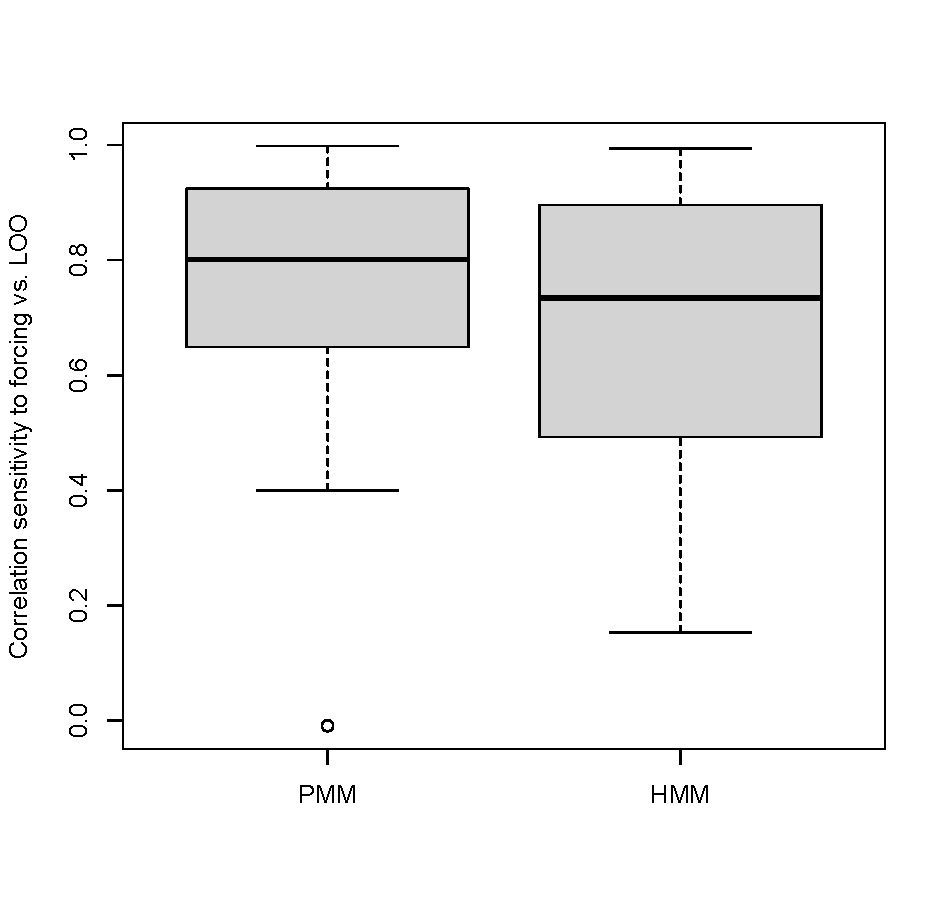
\includegraphics[width=0.7\textwidth]{../../analyses/phylogeny/figures/FigSXXX_LOO_cors_sensitivity_forcing.pdf}
  \caption{\textbf{Bias in estimation of sensitivity to environmental cues by non-phylogenetic vs. phylogenetic models.} Histograms show the difference between the phylogenetic model (PMM) with estimated $\lambda$ against the non-phylogenetic (HMM) model with $\lambda$ = 0, in their estimations of species sensitivities to three environmental cues: chilling (a), forcing (b) and photoperiod (c). Positive values indicate that sensitivities estimated by the non-phylogenetic model are smaller than those estimated by the phylogenetic model.}
  \label{fig:LOCO_slopescors}
\end{figure}


\end{document}
